\par{For a fully optimised algorithm, the aim is to have all of 
    the available hardware threads busy at all times. Once again, 
    this was never the case. Figure \ref{Concurrency_64_Phi} gives a breakdown 
    of the amount of time spent using a certain number of hardware threads. 
    It is clear that a large part of the execution time is spent with a 
    very low number of active threads. There is some good utilisation 
    of the hardware threads, which is likely to be due to the high number 
    of \emph{work groups} in executions of the internal kernel. The algorithm 
    needs to be modified in order to fully exploit the parallelism 
    available on the Xeon Phi.}

\begin{figure}[!h]
    \centering
    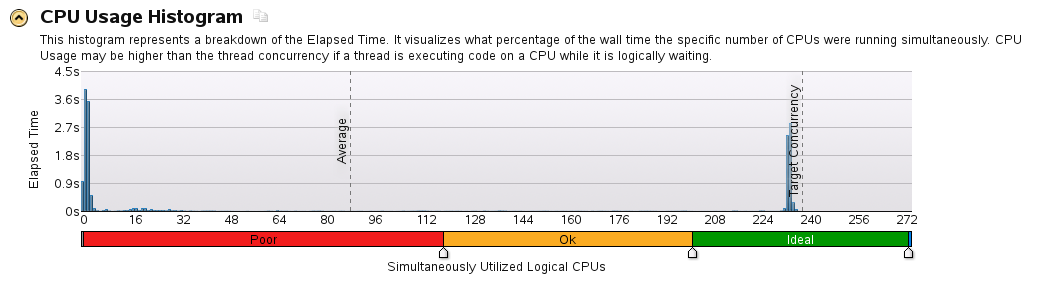
\includegraphics[width=1.0\textwidth]{figures/Concurrency_64_Phi.png}
    \caption{Concurrency on Xeon Phi with block size 64.}
    \label{Concurrency_64_Phi}
\end{figure}

